\section{Применение в высокоуровневом рендеринге}
В данной главе представлена имплементация высокоуровнего рендерера в целях тестирования дизайна и реализации RHI. Современный высокоуровневый рендерер должен быть модульным, удобным в использовании, а также в идеальном случае быть полностью конфигурируемым, включая возможность написания кастомного решения специально под нужды конкретного игрового проекта.

\subsection{Общий дизайн}
Дизайн, представленный в данной работе (см. рисунок \ref{fig:renderer_design}) стремится решить все эти проблемы. Рендерер состоит из абстрактных компонент -- IRenderFeature. Каждая из них декларирует вершины рендер графа, а также ECS системы (в основном предназначенные для агрегирования данных из компонент сущностей на сцене). Коммуникация между различными IRenderFeature сделана через абстрактный Context, способный содержать произвольные данные.

\begin{figure}[h]
    \centering
    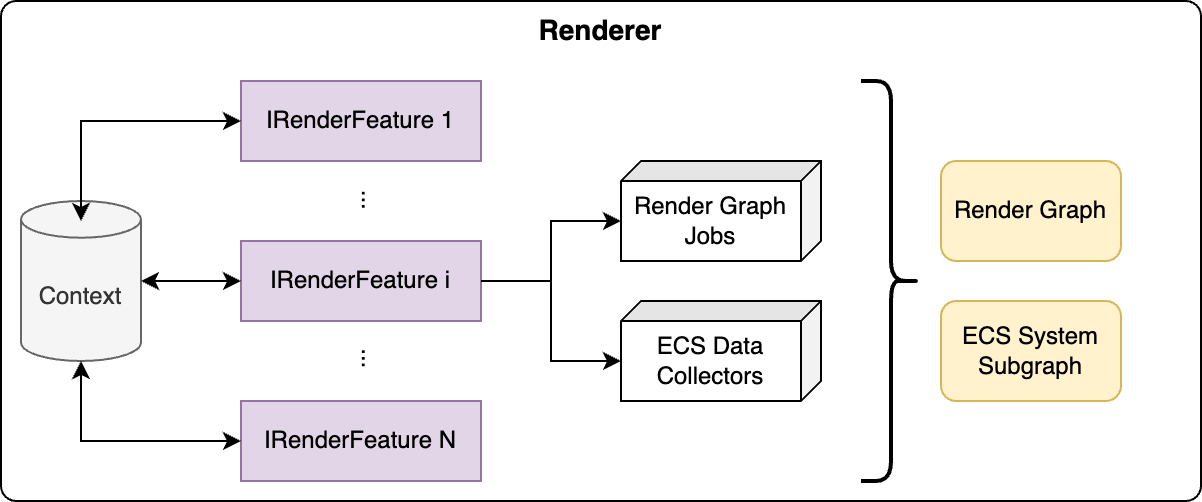
\includegraphics[scale=0.33]{renderer/renderer.png}
    \caption{Дизайн рендерера}
    \label{fig:renderer_design}
\end{figure}

Конкретные имплементации IRenderFeature можно классифицировать на: отрисовку геометрии, отрисовку процедурных объектов, а также эффекты постобработки. Поэтому в качестве рендерера по-умолчанию были реализованы методы рендеринга из всех данных классов в качестве проверки дизайна. Список реализованных IRenderFeature и вершины графа каждой из них представлены схематично на \ref{fig:built_in_renderer}.

\begin{figure}[h]
    \centering
    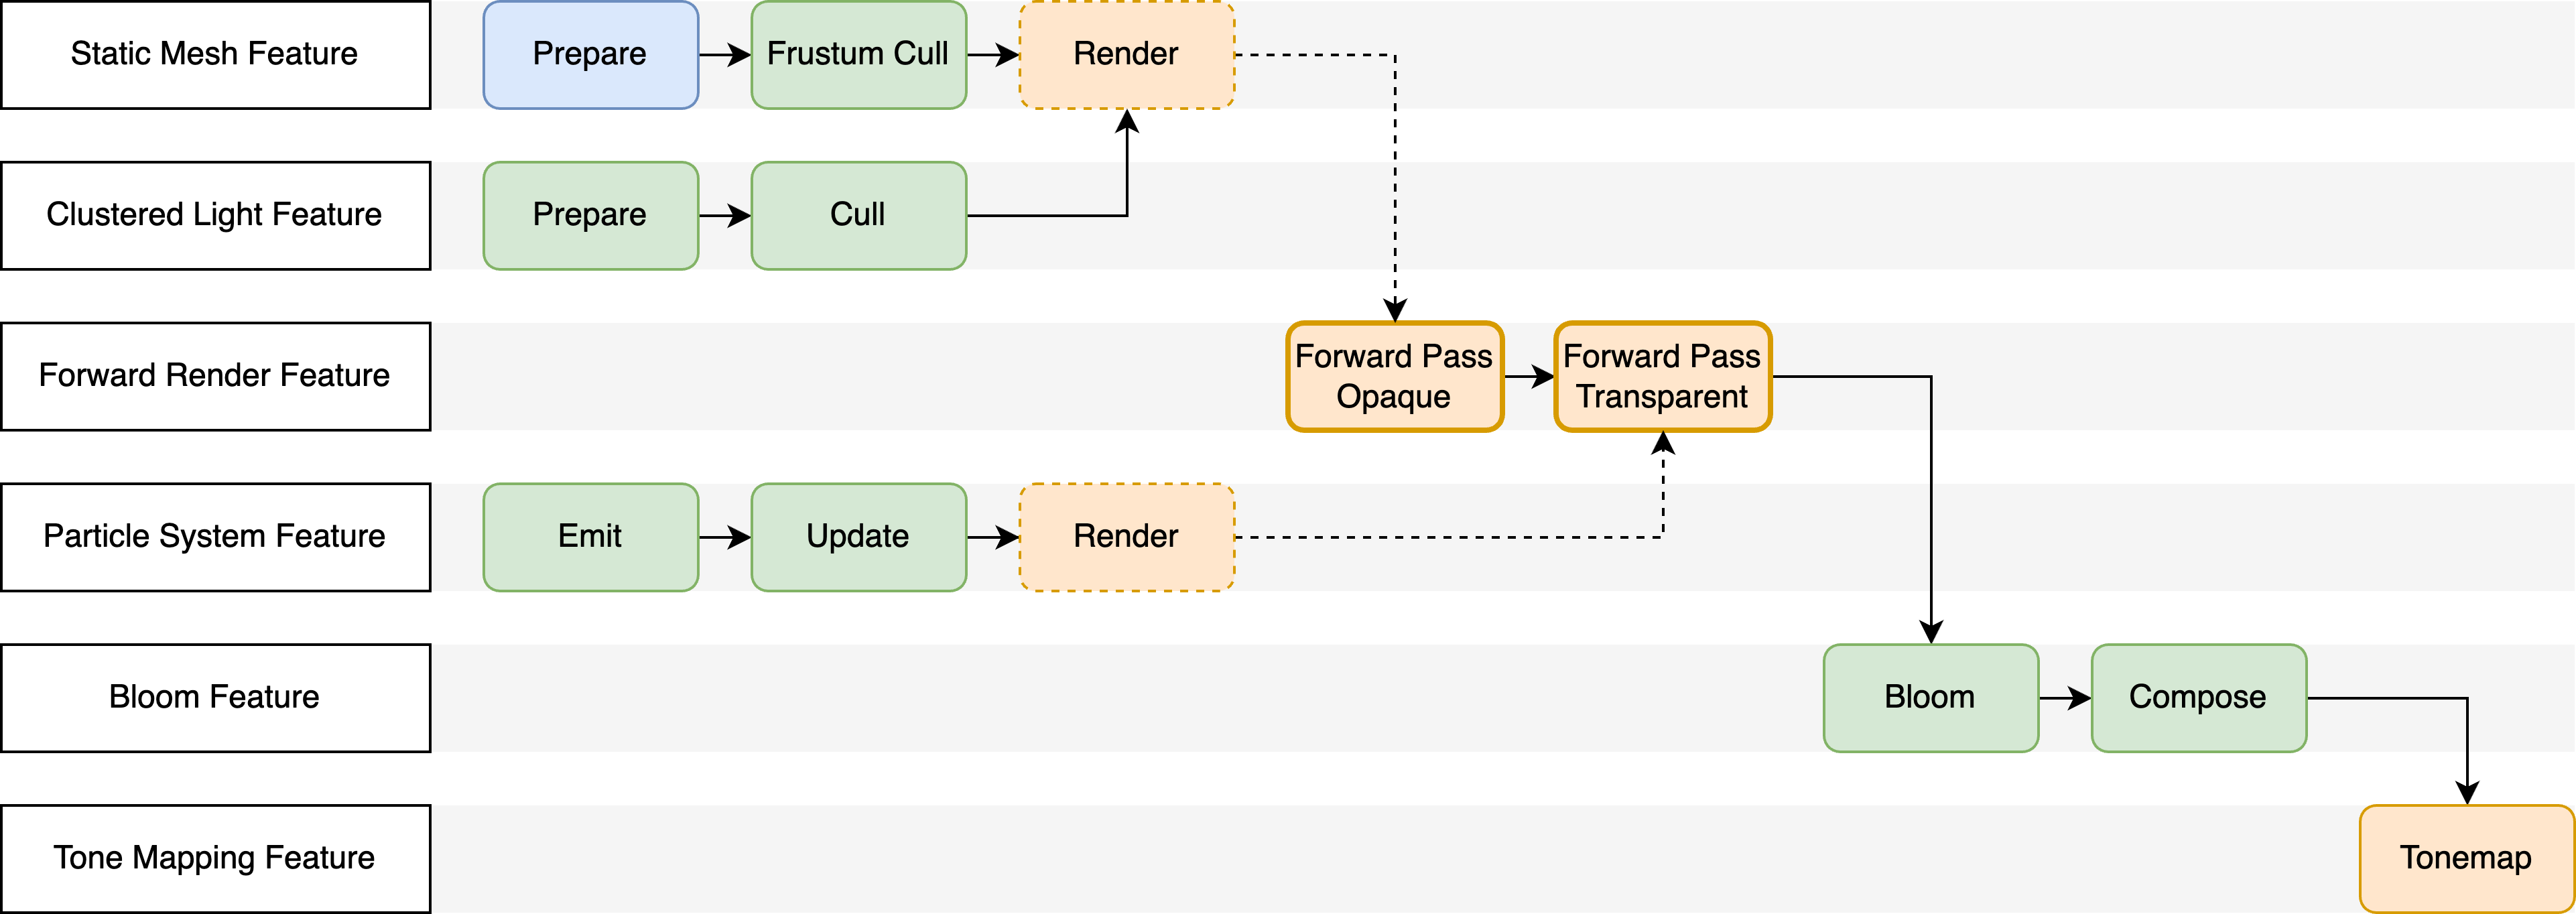
\includegraphics[scale=0.121]{renderer/built_in_renderer.png}
    \caption{Схема имплементации рендерера, представленной в данной работе далее.}
    \label{fig:built_in_renderer}
\end{figure}

\subsection{Отрисовка геометрии}
Еще до появления современных графических API, было стремление к так называемому GPU-Driven Rendering \cite{ubisoft_gpu_driven_rendering} (рендерингу, управляемому GPU), который представляет собой ряд решений, возлагающих значительную работу по генерации команд отрисовки напрямую на GPU. С увеличением комплексности сцен в видеоиграх, возникла необходимость в перераспределении задач таким образом, чтобы максимально использовать возможности GPU. Этот подход использует возможности параллельной обработки современных графических процессоров для выполнения таких задач, как отсеивание, сортировка и генерация вызовов отрисовки. Рендеринг геометрии -- основная цель данного метода. Поэтому было принято решение его задействовать.

У представленного метода два этапа -- отсечение по пирамиде видимости и растеризация видимой геометрии. Первый этап происходит в вычислительном шейдере, и помимо непосредственной проверки видимости каждого объекта он также генерирует косвенный буфер команд на GPU. Предположим, есть $N$ мешей, каждый из которых используется на сцене потенциально несколько раз. Соберем все экземпляры каждого меша в $N$ групп. Каждая группа будет одним непрямым вызовом отрисовки экземпляров. В командный буфер запишется лишь одна команда -- multi draw instanced indirect, которая на GPU будет представлена буфером из $N$ команд отрисовки. Заметим, что на центральном процессоре размер работы в таком методе довольно небольшой -- необходимо один раз разбить всю геометрию сцены на группы (препроцессинг), а дальше каждый кадр записать лишь две команды в командный буфер. Раньше вся эта работа (за исключением растеризации) происходила на CPU \cite{frustum_culling_2000}. Детальная схема описанного алгоритма представлена на рисунке \ref{fig:meshes_render}.

\begin{figure}[h]
    \centering
    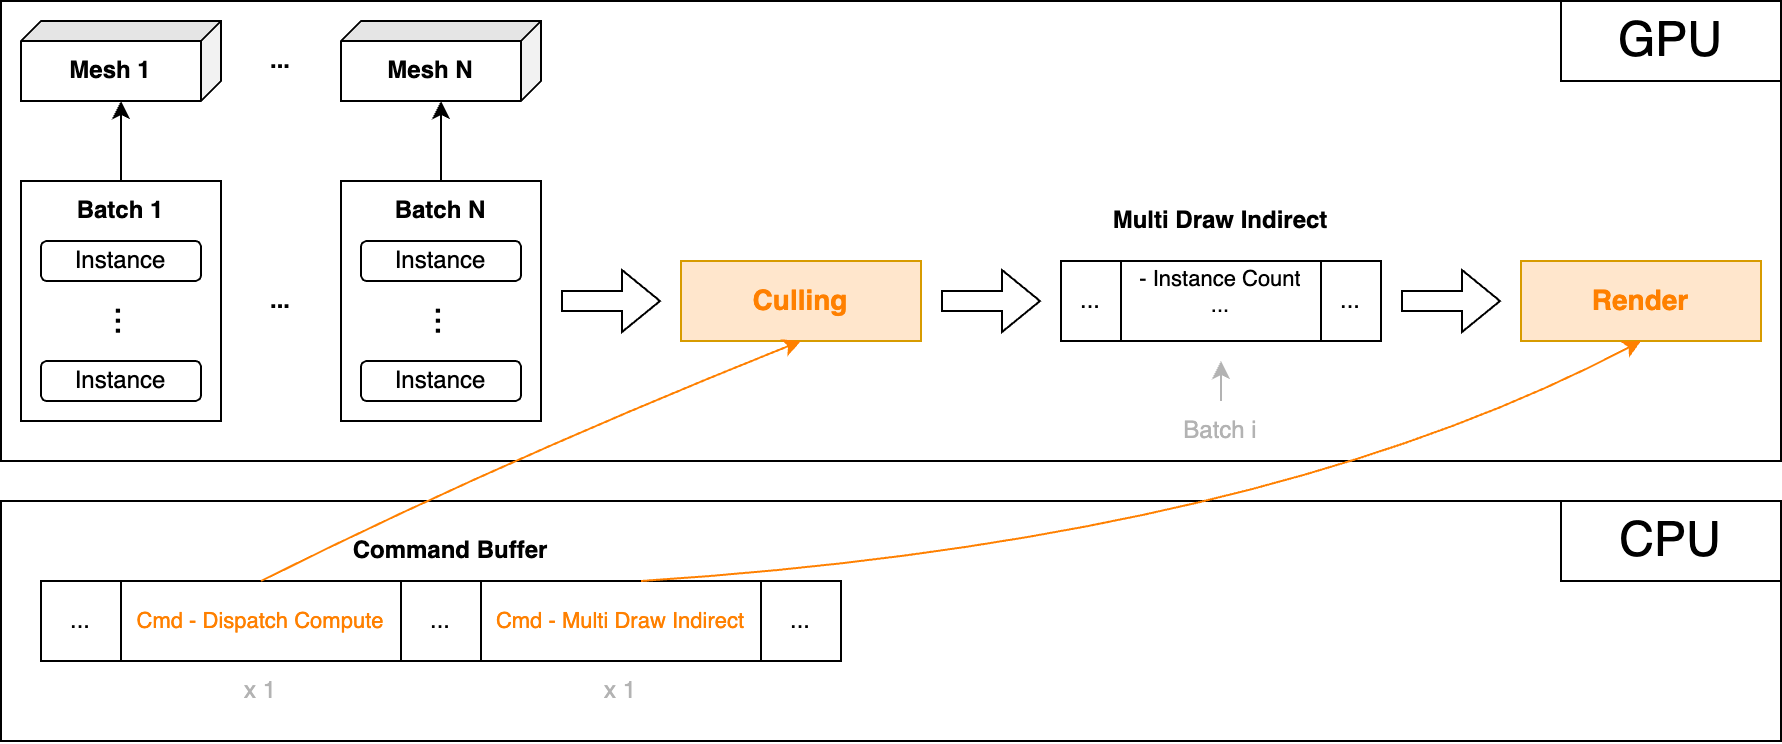
\includegraphics[scale=0.26]{renderer/meshes_render.png}
    \caption{Схема процесса рендеринга мешей.}
    \label{fig:meshes_render}
\end{figure}

При самой отрисовке используются техники физически корректного рендеринга (PBR) для достижения более визуально реалистичных результатов. PBR симулирует взаимодействие света с поверхностями в соответствии с физическими законами, что позволяет материалам выглядеть и вести себя как их реальные аналоги. Шейдерный код основан на решениях, представленных в \cite{pbr_book2016}.

\subsection{Кластерное отсечение света}
Одна из наиболее затратных (по объему необходимых вычислительных ресурсов) операций в графике является просчет освещения. Современные виртуальные сцены состоят из множества сложной геометрии и источников света. С физической точки зрения, свет, излучаемый источником света распространяется бесконечно далеко, однако в качестве вычислительной аппроксимации, учитывая что затухание света пропорционально $\frac{1}{d^2}$ (где $d$ -- расстояние от источника света), можно посчитать радиус точечного источника света, вне которого вклад будет пренебрежимо малым (см. коэффициент затухания \ref{eq:point_light_attenuation}; заметим, что $\text{Attenuation}(\text{LightRadius}) = 0$). Эта идея положила основу методам отсечения источников света \cite{Harada2012ForwardBD}, которые оптимизируют расчет освещения путем определения групп фрагментов, на которые не влияет определенный источник света.
\begin{align}
    \text{Attenuation}(d) \approx \frac{max \left(1 - \frac{d}{\text{LightRadius}}, 0\right) }{d^2}
    \label{eq:point_light_attenuation}
\end{align}

Метод кластерного отсечения света (clustered light culling) разделяет пирамиду видимости камеры на трехмерные кластеры, каждый из которых содержит информацию о всех источниках света, которые могут повлиять на пиксели в этом кластере. Кластеры расположены таким образом, что они полностью покрывают всю сцену и не пересекаются между собой. Для быстрой проверки пересечений для каждого кластера, то есть усеченной пирамиды, считается минимальный параллельный осям ограничивающий параллелепипед (англ. axis-aligned bounding box или AABB), содержащий весь объем кластера. Ограничивающий же объем для точечных источников света -- сфера.

\begin{figure}[h]
    \centering
    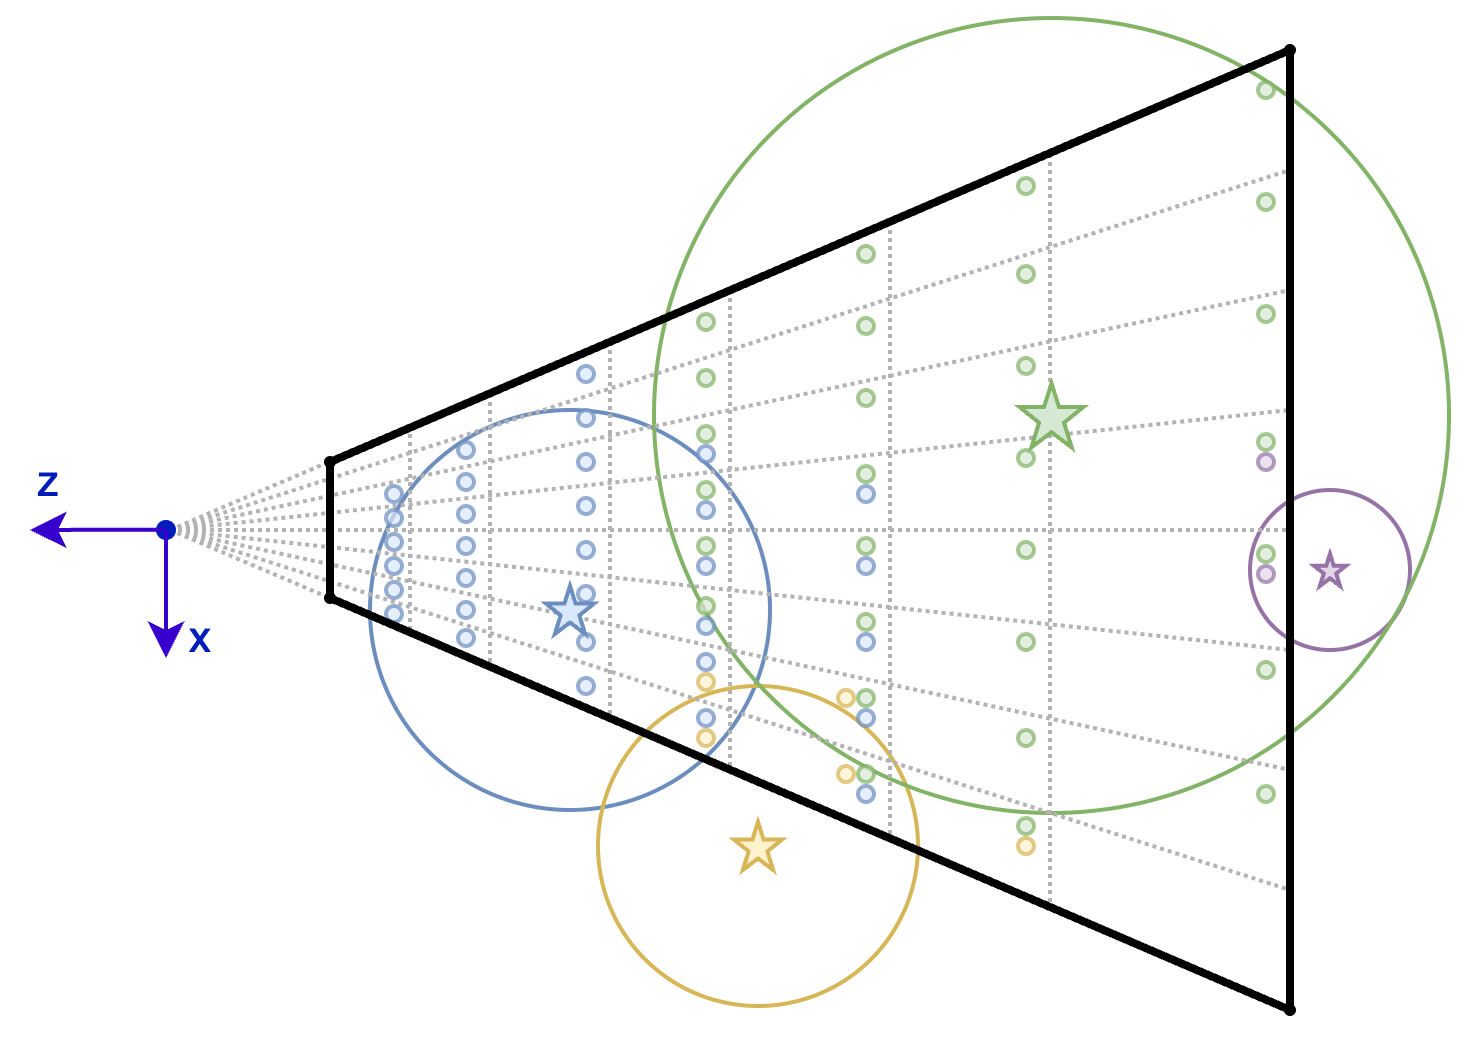
\includegraphics[scale=0.25]{renderer/clustered_light_culling_frustum_xz.png}
    \caption{Отсечение точечных источников света относительно трехмерных кластеров (вид в проекции на плоскость X-Z)}
    \label{fig:clustered_light_culling_frustum_xz}
\end{figure}

Существует несколько способов разбиения на кластеры. Дальше представлено разбиение, основанное на работе \cite{original_clustered_light_culling}. В плоскости X-Y экран разбивается равномерно на ячейки одинакового размера (в данной работе -- 16x16 пикселей). По глубине (вдоль оси Z) же пирамида разделяется экспоненциально, однако была выбрана более простая вычислительно аппроксимация разделения, представленная в докладе \cite{doom_clustered_z_splitting}:
\begin{align}
    z = \text{Near} \cdot \left( \frac{\text{Far}}{\text{Near}} \right) ^ {\text{SliceIndex} / \text{NumSlices}}
\end{align}

Данный алгоритм работает в два этапа -- построение ограничивающих объемов кластеров и непосредственное отсечение света. Первый шаг достаточно выполнять лишь при изменении размеров экрана, то есть когда пирамида видимости изменяется по форме. Второй шаг необходимо выполнять каждый раз когда изменяется положение и/или ориентация камеры, а также при движении источников света. Поскольку в современных видеоиграх преобладает непрерывная динамичность, на практике отсечение света вычисляется каждый кадр. Вызов вычислительного шейдера производится по количеству кластеров по соответствующим трехмерным индексам, то есть одна рабочая группа соответствует одному кластеру. Внутри рабочей группы каждый поток проверяет пересечения данного кластера с $\frac{\text{NumLights}}{\text{WorkGroupSize}}$ источниками света. По итогу внутри рабочей группы соберется полный список источников света (а точнее их индексов, для сокращения необходимой алгоритму видеопамяти), влияющих на данный кластер. Дальше этот список переносится из shared memory в глобальный буфер, который в последствии будет использоваться при подсчете освещения.

Помимо самого алгоритма, также была реализована отладочная визуализация комплексности освещения, которая отображается поверх просчитанного изображения. На каждый фрагмент добавляется цвет, показывающий как много источников света было обработано в расчете освещения данного фрагмента. Эта визуализация полезна не только для отладки работы представленного алгоритма, но также и для работы дизайнеров сцен, которые могут благодаря ней оптимизировать расстановку источников света, избегая большого количества пересечений источников света.

\subsection{Симуляция и отрисовка частиц}
Системы частиц являются важным компонентом компьютерной графики, используемым для моделирования таких явлений, как огонь, дым, дождь, взрывы и др. Традиционно эти системы обрабатывались на центральном процессоре \cite{lucasfilm_particle_systems_1983}. Это включало вычисление позиции, скорости и других свойств каждой частицы в системе для каждого кадра. CPU выполнял все необходимые физические расчеты, включая силы, такие как гравитация, ветер и столкновения. Однако ранние реализации систем частиц были вынуждены использовать упрощенную физику, методы рендеринга и малое количество частиц для достижения желаемых визуальных эффектов в рамках ограничений вычислительной мощности CPU, поскольку CPU не предназначены для высоко параллельной природы симуляций. Появление вычислительных шейдеров привело к переносу значительной части этой работы на GPU.

Симуляция частиц использует параллельную архитектуру GPU для обработки всего жизненного цикла частиц, от их "рождения" до "смерти". Подробная диаграмма системы частиц изображена на рисунке \ref{fig:particle_system_simulation_and_render}. Алгоритм разбит на три части:
\begin{enumerate}
    \item Emission (инициализация): в вычислительном шейдере "излучаются" новые частицы и инициализируются их атрибуты, такие как положение, скорость, цвет и время жизни. Поскольку на GPU нет динамических массивов, используется один буфер фиксированного размера со всеми частицами. Для определения, какие элементы (частицы) этого буфера свободны, используется вспомогательный буфер -- free list.
    \item Simulation (симуляция): каждый кадр другой вычислительный шейдер обновляет атрибуты частиц на основе физических расчетов. Это может включать применение сил, обновление скоростей и проверку на столкновения. В случае, если время жизни частицы закончилось, ее индекс добавляется в free list. Также, на этом этапе происходит запись индексов действующих и видимых частиц в еще один вспомогательный буфер.
    \item Rendering (отрисовка): как и при отрисовке мешей здесь используется метод GPU-driven rendering. Этап симуляции генерирует команду отрисовки на GPU, где instance count равен числу действующих и видимых частиц. В качестве геометрии для отрисовки используются четырехугольники, ориентированные в сторону камеры \cite{schaufler1995dynamically}, на которые потенциально накладывается текстурный атлас (по времени жизни выбирается текущая текстура).
\end{enumerate}

\begin{figure}[h]
    \centering
    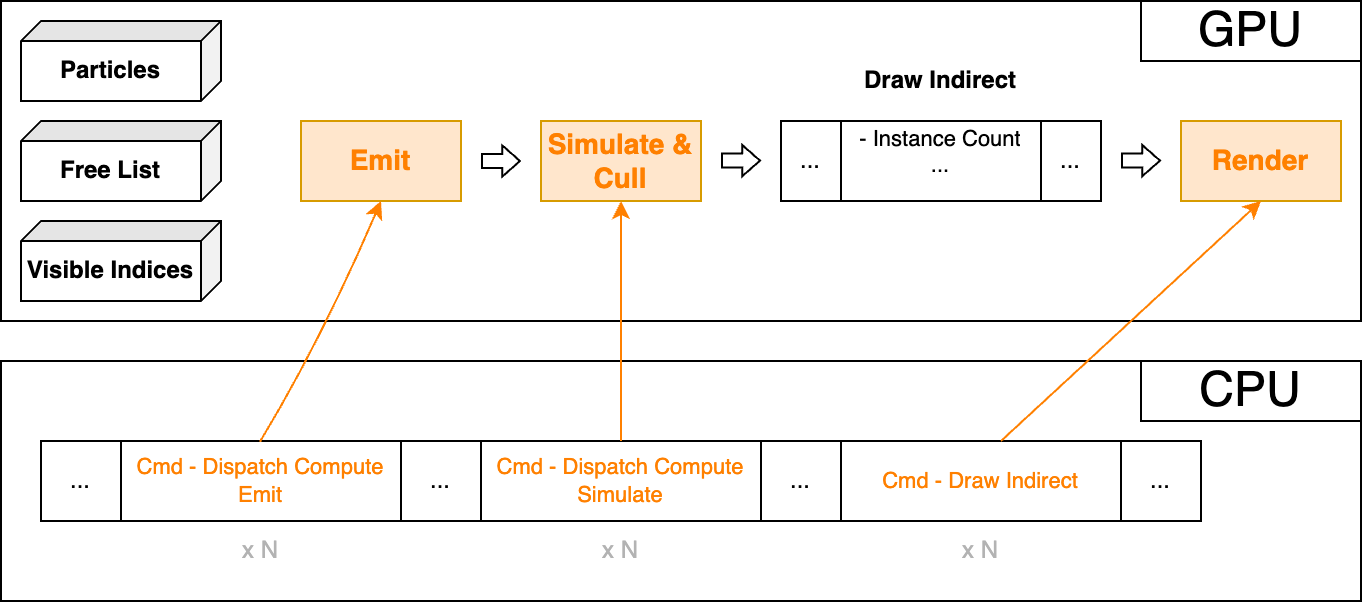
\includegraphics[scale=0.3]{renderer/particle_system_simulation_and_render.png}
    \caption{Схема процесса симуляции и рендеринга частиц}
    \label{fig:particle_system_simulation_and_render}
\end{figure}

\subsection{Эффекты постобработки}
Следующим концептуально отличающимся элементом рендерера является стек эффектов постобработки. Данные эффекты преобразуют уже отрендеренное изображение. В данной работе были реализованы два эффекта -- bloom и tone mapping.

\subsubsection{Bloom}
Эффект свечения (bloom) является популярной техникой постобработки, используемой для имитации рассеивания яркого света в человеческом глазу, создавая светящийся ореол вокруг ярких областей изображения. Этот эффект улучшает реалистичность сцен, особенно тех, которые включают интенсивные источники света, такие как солнце, огни или отражающие поверхности. Для данного эффекта необходимо, чтобы входное изображение было с высоким динамическим диапазоном (HDR), где контраст между яркими и темными областями более выражен.

Алгоритм генерации данного эффекта был взят из доклада \cite{cod_aw_bloom} и состоит из сначала последовательного downsampling, используя кастомный фильтр (см. рисунок \ref{fig:bloom_downsample}), который был придуман для борьбы с негативными темпоральными артефактами, а потом последовательного аддитивного upsampling с тент-фильтром размера 3x3 (см. формулу \ref{eq:tent3x3}) и композиции. Схематично этапы работы алгоритма представлены на рисунке \ref{fig:bloom_diagram}.

\begin{align}
    \text{T} = \frac{1}{16} \begin{bmatrix}
                                1 & 2 & 1 \\[0.1em]
                                2 & 4 & 2 \\[0.1em]
                                1 & 2 & 1
                            \end{bmatrix} \label{eq:tent3x3}
\end{align}

\begin{figure}[h]
    \centering
    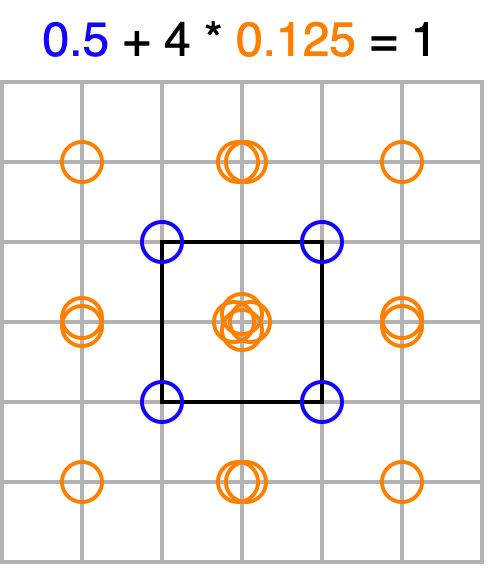
\includegraphics[scale=0.26]{renderer/bloom_downsample.png}
    \caption{Кастомный downsample, митигирующий негативные темпоральные артефакты.}
    \label{fig:bloom_downsample}
\end{figure}

\begin{figure}[h]
    \centering
    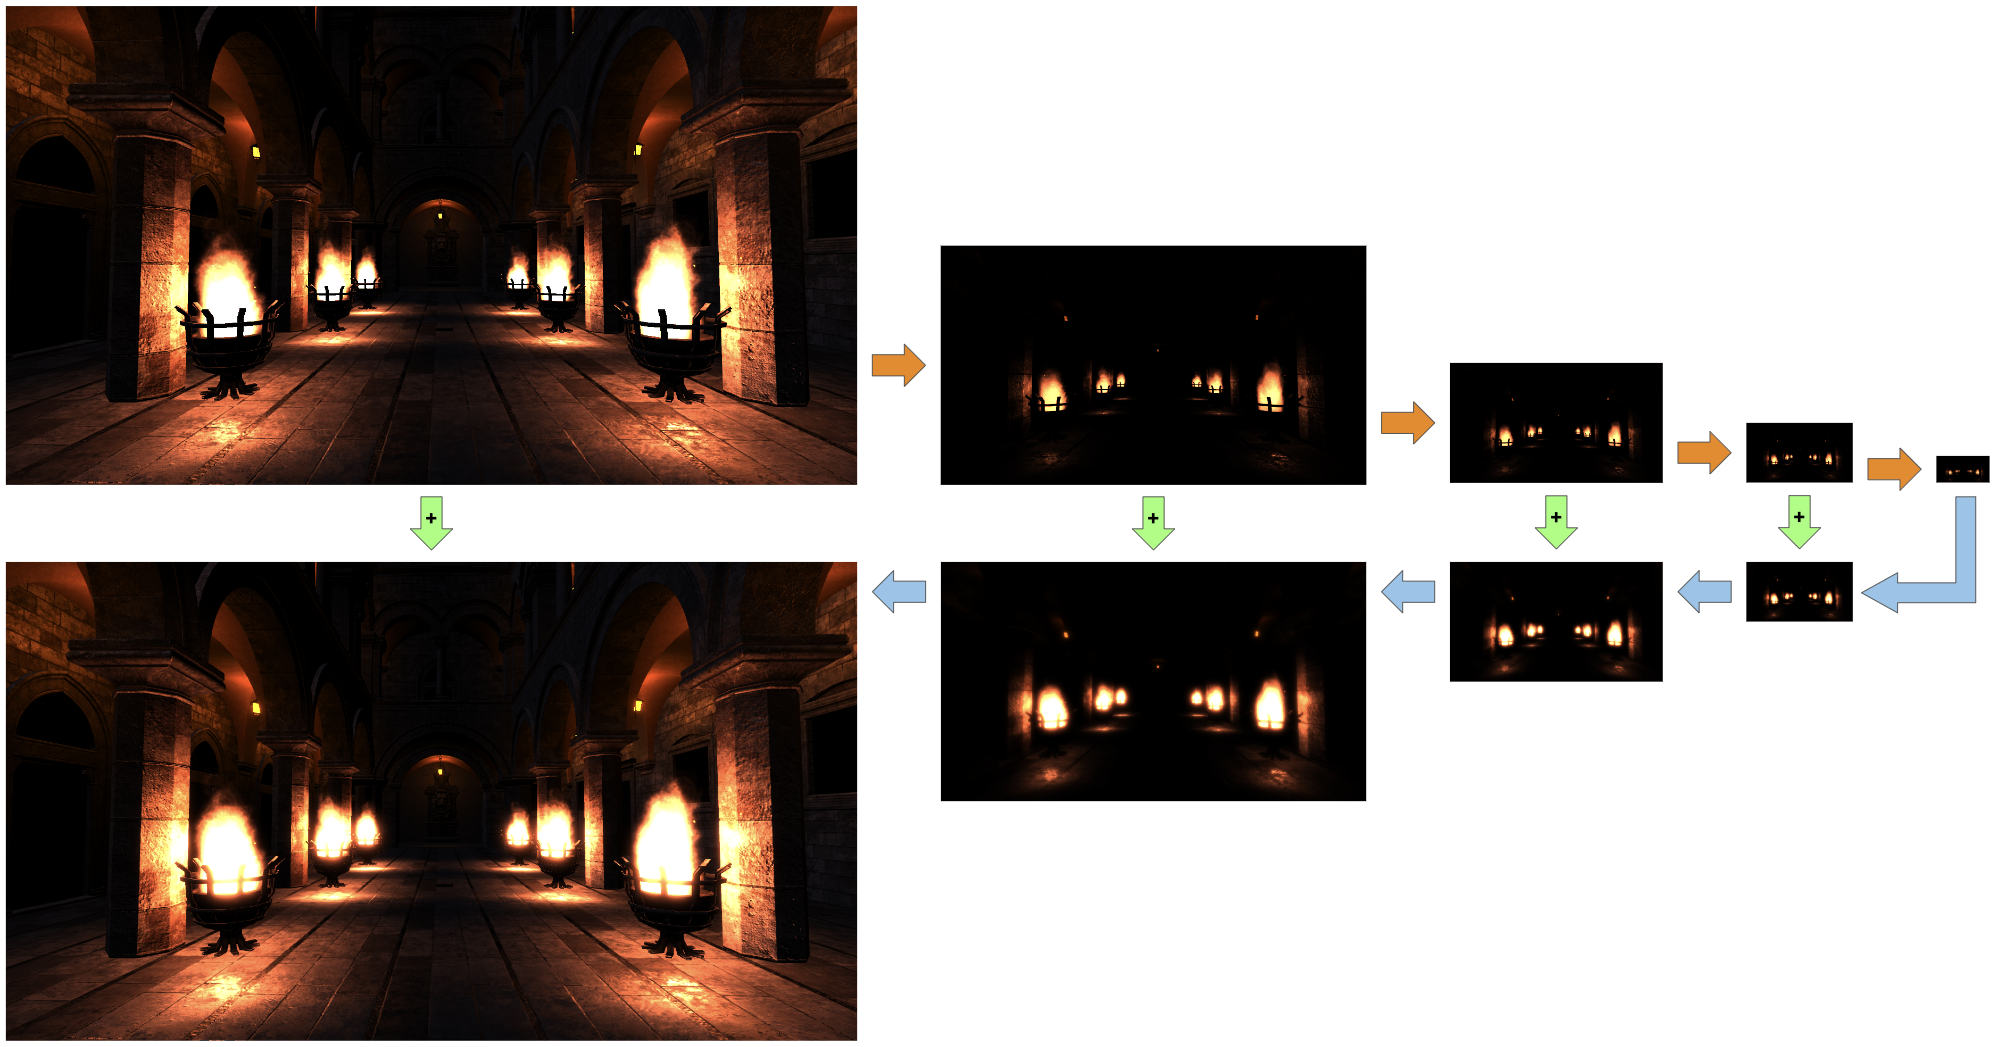
\includegraphics[scale=0.23]{renderer/bloom_diagram.png}
    \caption{Схема просчета эффекта свечения. Изображения представлены без применения tone mapping.}
    \label{fig:bloom_diagram}
\end{figure}

Первый downsampling отличается от последующих. На нем кастомный фильтр считается по взвешенным средним использованных семплов \cite{karis2014}, используя luma: $w(L_\text{HDR}) = \frac{1}{1 + \text{luma}\left( L_\text{HDR} \right)}$, где $\text{luma}\left( v \right) = dot\left( (0.2126, 0.7152, 0.0722), v^{-2.2} \right)$, а после этого происходит отделение только "ярких" частей, что сделано для возможности художественной конфигурации эффекта при помощи параметров $t$ (\textit{threshold}) и $s$ (\textit{soft threshold}):

\begin{align}
    B( c ) &= max( c.r, c.g, c.b ) & \text{яркость}&\\
    S( c ) &= \frac{ ( clamp( B( c ) - t + t s,  0,  2 t s ) )^2 }{ 4 \cdot (t s + bias) } & \text{смягчающая кривая}&\\
    P( c ) &= c \cdot \frac{ max( S (B(c)), B(c) - t ) }{max(B(c), bias)} & \text{результат префильтрации}\label{eq:bloom_prefilter_config}
\end{align}

\subsubsection{Tone mapping}
Тональное отображение (англ. tone mapping) является ключевым процессом в рендеринге с высоким динамическим диапазоном (HDR), позволяющим преобразовать изображения, которые имеют широкий диапазон значений яркости, в формат, подходящий для отображения на стандартных дисплеях с ограниченным динамическим диапазоном. В данной работе реализовано тональное отображение на основе экспозиции \cite{tone_mapping}, динамически регулирующее экспозицию различных областей изображения для сохранения деталей по всему спектру яркости, обеспечивая видимость и правильное отображение как теней, так и высветлений (см. рисунки \ref{fig:tone_map_vis}). Формула отображения представлена ниже:
\begin{align}
    L_{\text{mapped}}(x, y) = \left( 1, 1, 1 \right) - e^{-L_{\text{HDR}}(x, y) \cdot \text{exposure}}
\end{align}

\begin{figure}[h]
    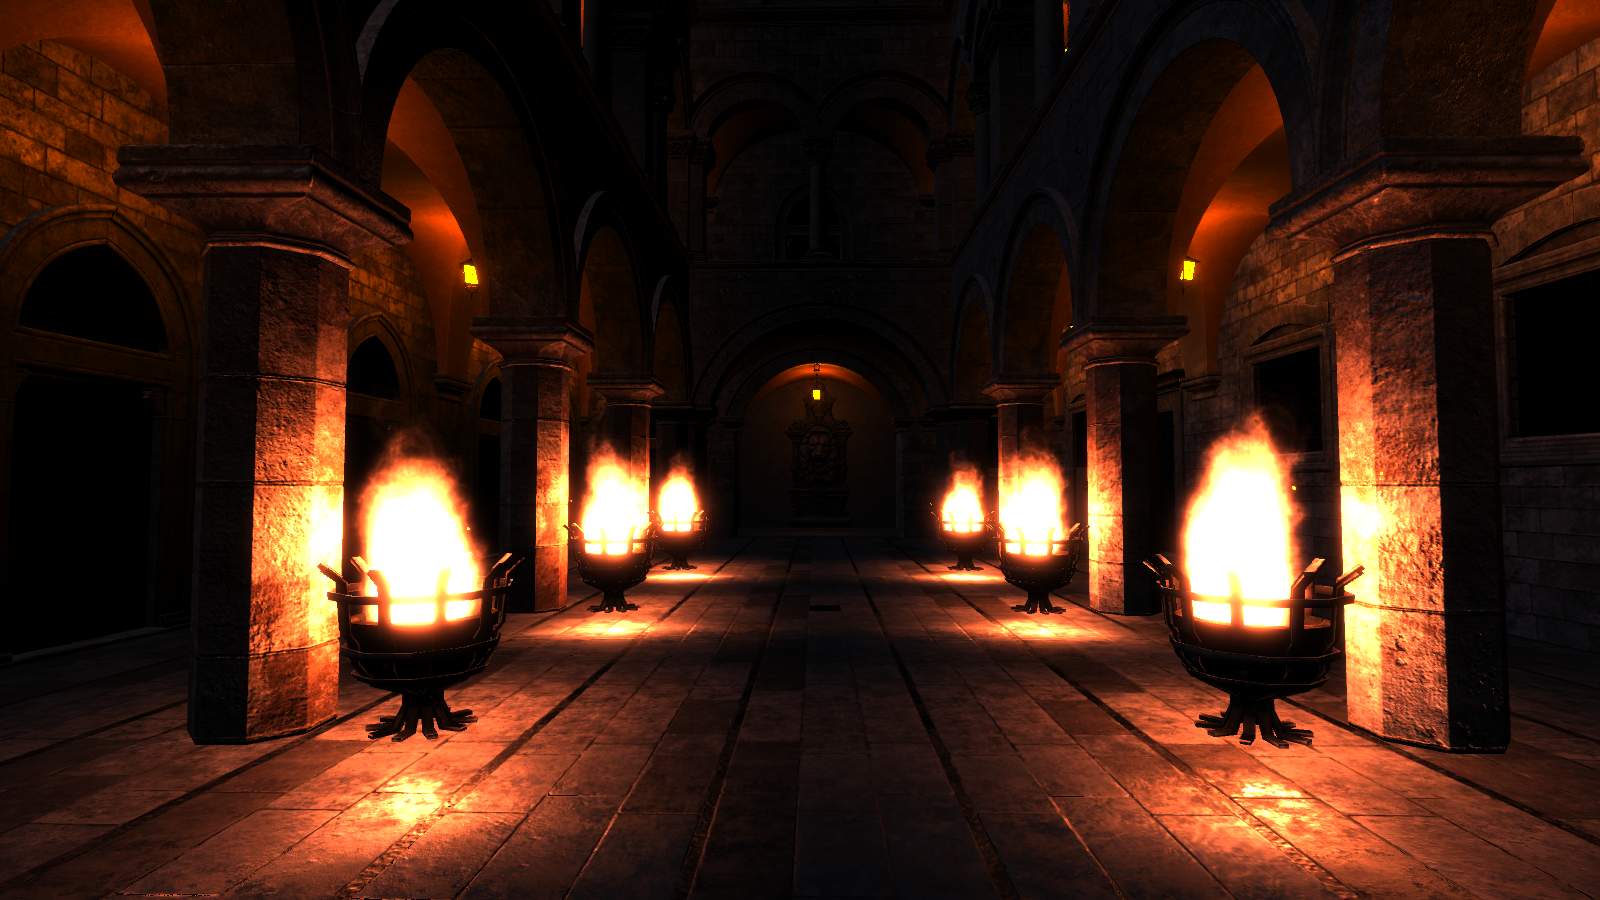
\includegraphics[scale=0.145]{renderer/pre_tonemap.png}
    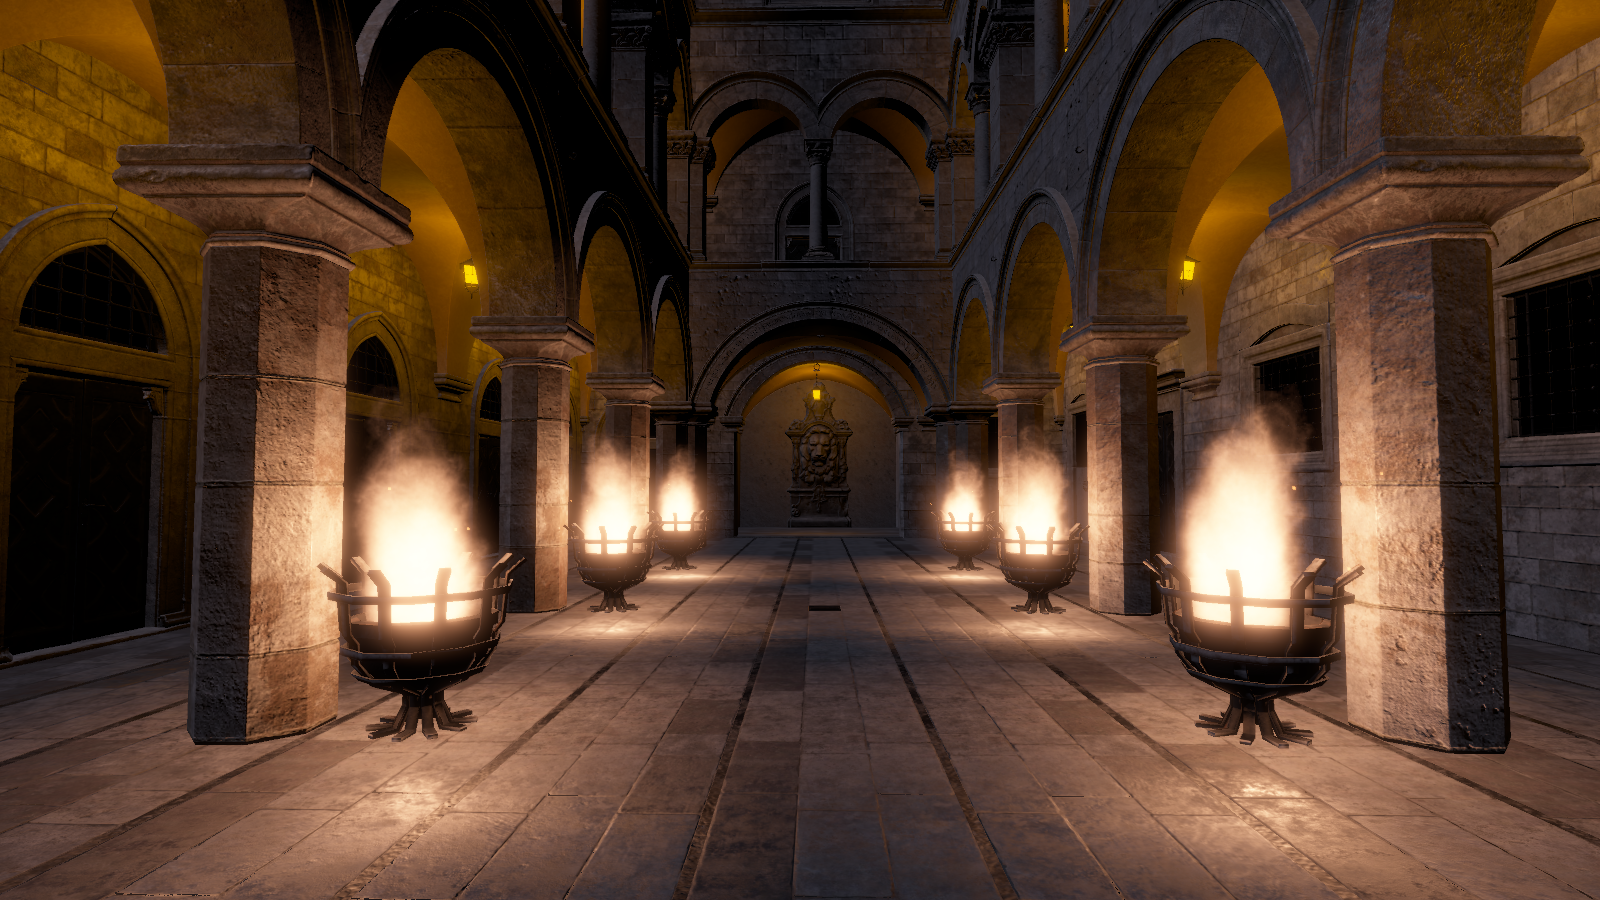
\includegraphics[scale=0.145]{renderer/post_tonemap.png}
    \caption{Визуализация тонального отображения с $\text{exposure} = 0.6$; слева направо: $L_{\text{HDR}}(x, y)$ и $L_{\text{mapped}}(x, y)$.}
    \label{fig:tone_map_vis}
\end{figure}

